\documentclass[11pt]{amsart}
\usepackage{geometry}                % See geometry.pdf to learn the layout options. There are lots.
\geometry{letterpaper}                   % ... or a4paper or a5paper or ... 
%\geometry{landscape}                % Activate for for rotated page geometry
%\usepackage[parfill]{parskip}    % Activate to begin paragraphs with an empty line rather than an indent
\usepackage{graphicx}
\usepackage{amssymb}
\usepackage{epstopdf}
\usepackage{parskip}
\usepackage{setspace} 
\usepackage{algorithm}
\usepackage{algpseudocode}
\usepackage{enumitem}
\setlength{\parindent}{12pt}

\DeclareGraphicsRule{.tif}{png}{.png}{`convert #1 `dirname #1`/`basename #1 .tif`.png}

\title{Data Preprocessing}
\author{The Author}
%\date{}                                           % Activate to display a given date or no date
\begin{document}
\begin{spacing}{1.1}

\maketitle
%\section{}
%\subsection{}
The Dynamic Time Warping(DTW) algorithm is the one of the oldest algorithms that is used to compare and cluster sequences varying in time, length and speed. Formally, given two temporal sequences, the algorithm utilises the technique of dynamic programming to find an optimum alignment between  through the computation of local distances between the points in each sequence. The time and computational complexity of this algorithm is  \emph{O}(mn) where $m$ and $n$ denote the length of the sequences that are being compared. Thus for  high dimensional time series sequences, the time and computational costs incurred by the algorithm are quite high which  makes DTW a very unattractive choice for clustering or discovering motifs in high dimensional  data sets.  Intuitively speaking, DTW is a clustering algorithm that clusters similar patterns varying in time and speed. Another drawback for working in high-dimensional spaces is the contrast between the distances of nearest and furthest points. The distances between such points  become increasingly smaller  as the dimensionality increases. This makes it  difficult to construct meaningful cluster groups in such spaces.

To address the issue of the curse of dimensionality, DTW algorithms employ a window constraint to reduce the search space. The window constraints determine the allowable  shapes that a warping path can take. As the dimensionality of the data increases, the size of the window is adjusted accordingly. Rigid  window constraints impose a more rigid alignment  that prevent an overly temporal skew between two sequences, by keeping frames of one sequence  from getting too far from the other. For clustering data sets such as speech utterances, the effect produced by such global constraints is highly undesirable. If we consider two utterances of a word spoken at different time frames, the patterns can have an overly temporal askew between them as result of the different contexts in which the  words are spoken and/or as a result of  different speakers speaking the same word. Thus it is necessary to explore techniques  other than window constraints that can improve the performance of the DTW algorithm in terms of both accuracy and time. 

 Before investigating methods to improve a technique, it is highly necessary to first understand the nature of the data itself. In this chapter, I investigate data-driven preprocessing techniques  that attempt to understand the underlying intrinsic structure of the lower-dimensional space on which the  data lives. By achieving a thorough understanding of the data,we can   achieve dimensionality reduction by  isolating and identifying smaller set of new(current)  features  that are more relevant for the problem in hand. 
 
 
 There are presently two groups of preprocessing techniques commonly used to address this issue:
\begin{itemize}
\item  Feature Selection 
\item Feature Extraction
\end{itemize}
 Feature selection techniques  involve selecting only a subset of attributes from the original data.  One of the most popular approaches to feature selection is  the exploratory data analysis(EDA). EDA is an approach to data analysis that postpones the usual assumptions about what kind of model the data follows with the more direct approach of allowing the data itself to reveal its underlying structure and models. The particular techniques employed in EDA are often quite simple, consisting of various techniques of:
 
 \begin{enumerate}
\item Plotting the raw data (such as data traces, histograms, histograms, probability plots, lag plots, block plots, and Youden plots.
\item Plotting simple statistics such as mean plots, standard deviation plots, box plots, and main effects plots of the raw data.
\item Positioning such plots so as to maximize our natural pattern-recognition abilities, such as using multiple plots per page.
 \end{enumerate}
Feature extraction processes on the other hand are concerned with  a range of techniques  that apply an appropriate functional mapping to the original attributes to extract new features. The intuition behind feature extraction is that the data vectors $\{x_n\}$ typically lie close to a non- linear manifold whose intrinsic dimensionality is smaller than that of the input space as a result of strong correlations between the input features. Hence by using appropriate functional mapping, we obtain a smaller set of features that capture the intrinsic correlation between the input variable. Hence by doing so, we move from working in high dimensional spaces to working in low dimensional spaces. The choice  of appropriate functional mapping can  also improve the clustering of data as shown by figure 1:

In the rest of this chapter,  I explore a range of  feature selection and extraction methods  and investigate whether their application can improve the performance of the DTW algorithm in terms of both accuracy and time complexity.

\begin{figure}[h]
  \centering
   
     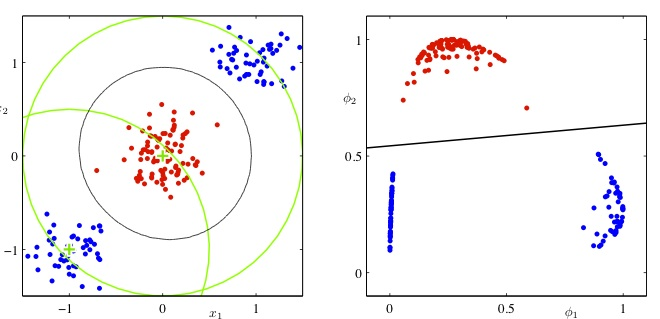
\includegraphics[scale=0.8]{featuremapping.jpg}
  \caption{The figure on the right corresponds to location of the data points in the feature space spanned by gaussian basis functions $\phi_1(x)$ and $\phi_2(x)$ }
  
\end{figure}
\newline
%The DTW algorithm combined  with the  1 nearest neighbour classifier  is a memory based algorithm. Memory-based methods involve storing the entire training set in order to make predictions for future data points. They typically require a metric to be defined that measures the similarity of any two vectors in input space, and are generally fast to �train� but slow at making predictions for test data points. The time and computational complexity associated with such methods is even higher when the dimensionality of the data points is high. Intuitively speaking, DTW is a clustering algorithm that clusters similar patterns varying in time and speed. In high- dimensional spaces, however, the contrast between the nearest and furthest points gets increasingly smaller, making it difficult to construct meaningful cluster groups. To address this issue, data dimensionality methods are used at the  preprocessing stage.
 
\section{Feature Selection}
The computational and time complexity associated with the DTW algorithm is governed by the dimensionality of the time  series. To get a feel of the data, I employed exploratory data analysis on the  isolated word utterances belonging to the test and training data sets  that I constructed from the TIDIGITS corpus. The aim here   to identify and isolate redundant features from the time series data.
 To get an idea about the structure of the data, I have studied the plots of the time series sequences along with performing auditory perception on the individual samples. Figure 2 gives the plot of raw signal corresponding to the word `8' by a speaker from the \emph{boy} category. From the visual and auditory analysis, I have made the following  observations:
\begin{itemize}
\item Long durations of silence occupy the beginning and end of each utterance.   These durations of silence segments are considerably long compared to the interesting regions in the acoustic signal that actually contain information about the spoken digit .  Removing these silence segments not only  reduce the dimensionality of the time series but also results in minimal loss of information.
\item  Through auditory perception of numerous samples, I have discovered that  the recordings are highly distorted when played in matlab even when the data is scaled so that the sound is played as loud as possible without clipping. The distorted signal fails to provide any time auditory clue about  category of the speaker i.e whether the speaker belongs to \{ boy,girl, men,women\}  and the signal must be played multiple times  for its class to be correctly identified.
\end{itemize}
\begin{figure}[h!]
  \centering
   
     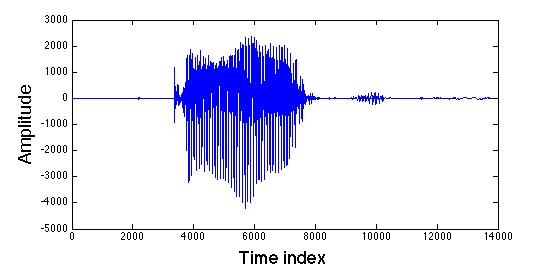
\includegraphics[scale=0.6]{Rawsample.jpg}
  \caption{`Raw 'signal}
  
\end{figure}
From  further experiments,  I have seen that if  I down-sample the utterances by $\frac{1}{2}$  which in other words means decreasing the sampling frequency by half, the resultant sampled signal is much clearer to understand. Sub-sampling  the utterances by half involves removing every other sample from the time series.  From the observation of figure 3, it can be sen that this technique  keeps the global trend of the signal intact but results in the  loss of local information. Furthermore through auditory perception of the sampled signals, I have discovered that losing some \textbf{local information} actually cleans the signal in a manner that allows the listener to identity the speaker's category and the utterance's class with ease.

With this knowledge  I have constructed  the following algorithm: `signal filter` that achieves  feature selection by removing segments of silence and downsampling the remaining segments by half.  An outline of the algorithm is as follows:

\begin{algorithm}[h]

\begin{algorithmic}[1]
\Procedure{SignalFilter}{$signal$}\Comment{raw signal }
\State $threshold=0$
\State maxAmplitude= max(rawSignal)
 \State Adapt the threshold based on the value taken by the maximum amplitude
 \State signalSil\_R$\leftarrow$ removeSilence(rawSignal,threshold)
 \State \textbf{return} output$\leftarrow$ downsample signalSil\_R by $\frac{1}{2}$
 
 \EndProcedure
\end{algorithmic}
 \caption{SignalFilter}
\end{algorithm} 
 \begin {itemize}
 \item The algorithm removes all samples in the times series sequence whose magnitude is less than the threshold. The threshold used is an adaptive parameter. By using the information of the signal's maximum amplitude the algorithm sets the threshold accordingly. It raises the threshold for signals corresponding to speakers having a loud and deep voice   and lowers the threshold for signals corresponding to speakers having gentle and low voice.
 \end{itemize}   
  
  
 \begin{figure}[H]
  \centering
   
     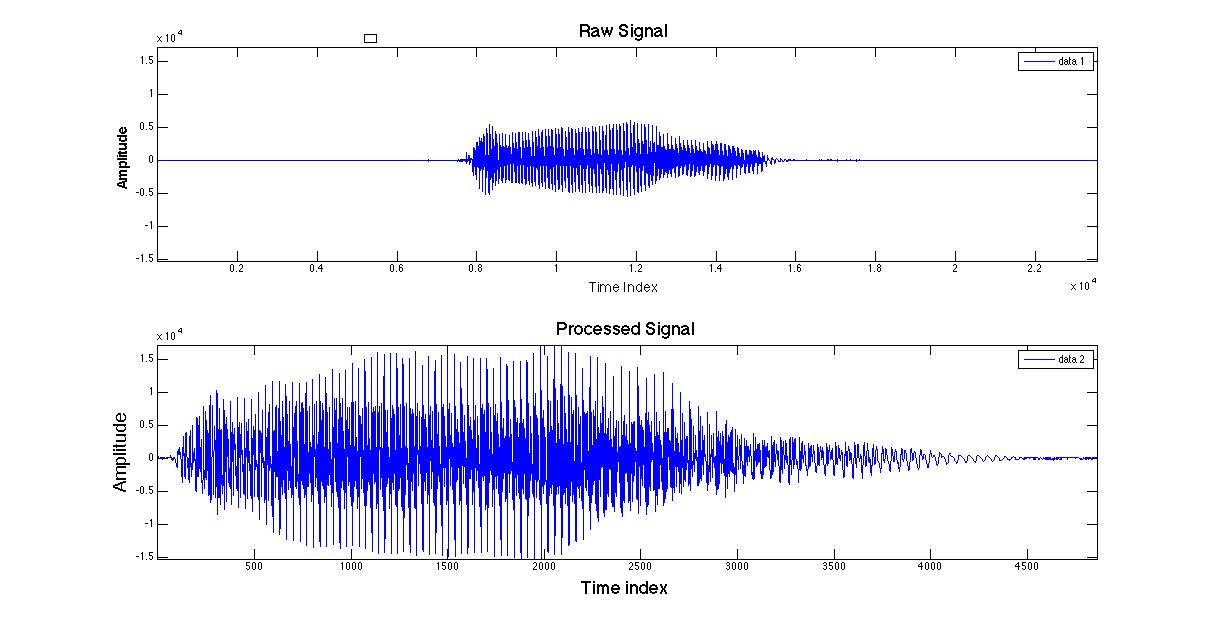
\includegraphics[scale=0.3]{Feature_selection.jpg}
  \caption{shows the raw acoustic signal corresponding to the utterances of the digit '5' alongside with the version that has its dimensionality reduced by the filter discussed above. From the comparison of the plots, it can be observed that the filter preserves the interesting patterns associated with the utterance while succeeding in reducing the dimensionality of the data.    }
  \end{figure}
  

 To analyse how introducing this feature selection process effects the performance of a DTW algorithm in working with high dimensional data, I have run the baseline value-added DTW(i.e DTW using raw values)  twice: once using the feature selection process as a preprocessing step and once without the feature selection process. An outline of the algorithm is given below.  
 \begin{algorithm}[H]

\begin{algorithmic}[1]
\Procedure{Value-based}{$seq1,seq2$}\Comment{two raw sequences }
 \State w = max($\lceil{0.1*max(n.m)}\rceil$, abs(n-m)) \Comment{Window constraint }
 \For{i=1: to length(seq1) }\Comment{Initialise the DTW cost matrix}
 \State DTW(i,0) = $\infty$
 \EndFor
 
 \For{i=1 to length(seq2)}
 \State DTW(0,i) = $\infty$
 \EndFor
 
  \For{i=2 to length(seq1)}  
 \For{j=max(2, i-w) to min(length(seq2), i+w)} \Comment { cost(a,b)$\equiv$euclid(a,b)}
 \State DTW(i,j) = cost(seq1(i),seq2(j)) + min\{ DTW(i-1,j)+DTW(i,j-1)+DTW(i-1,j-1)\}
 \EndFor
 
 \EndFor
\State \texbf{return}  result = $\frac{\mbox{DTW(n,m))}}{nm}$ \Comment{n=length(seq1), m=length(seq2)}

\EndProcedure} 
\end{algorithmic}
\caption{Value-Based DTW}
\end{algorithm}
 
 The focus of my research here is to improve the accuracy of the DTW algorithm while reducing the time and computational cost to a minimum. Even after applying the feature selection process the dimensionality of the time series sequences is still very high. Thus for these experiments I have employed the most rigid window constraint   w = max($\lceil{0.1*max(n.m)}\rceil$, abs(n-m)) that keeps frames from one sequence  from getting too far from the other. The results found from the experiments are as follows:
 \begin{figure}[H]
  \centering
   
     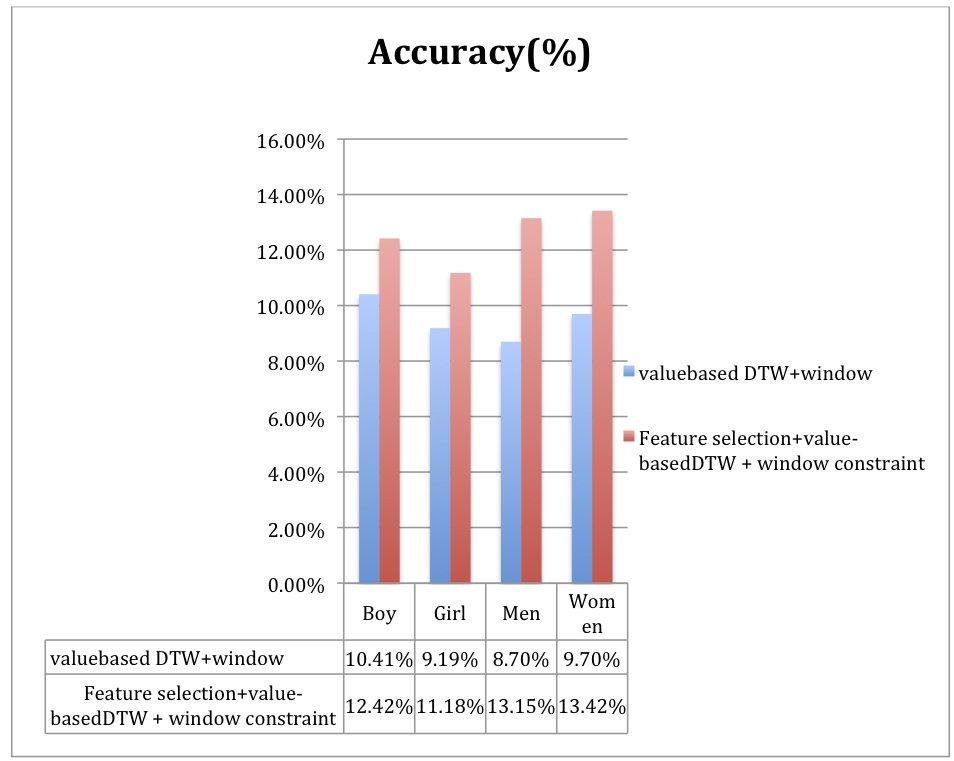
\includegraphics[scale=0.8]{value-basedaccuracy.jpg}
  \caption{ }
  
\end{figure}
\begin{figure}[H]
  \centering
   
     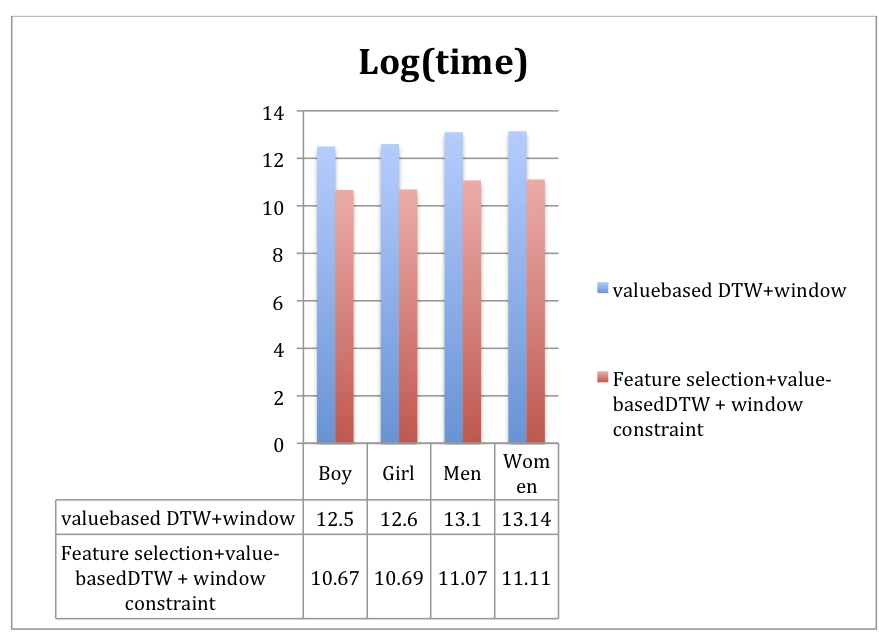
\includegraphics[scale=0.6]{value-basedtime.jpg}
  \caption{}
  
\end{figure}

Observations:
\begin{itemize}
\item Employing the prior feature selection process allows DTW subjected to global window constraint to improve both its accuracy and time complexity.

Explanations:
\begin{itemize}
 \item The DTW algorithm,due to  the high dimensionality of the  time series sequences is subjected to a window constraint that forces the algorithm to operate on the diagonal region of the DTW cost matrix. Removing  these redundant features increases the accuracy because these features  primarily represent segments of silence and since all utterances contain silence segments, taking these silences into account degrades the performance as  they bring i an unwanted notion of similarity in dissimilar patterns.
\item The size of the DTW cost matrix is \emph{O}(mn). Achieving dimensionality reduction through feature selection reduces the size of the cost matrix and thus decreases the computational cost.
\end{itemize}
\end{itemize}
\section{Feature extraction}
To improve the performance of the DTW algorithm even further, in this section I investigate domain-independent and domain dependent feature extraction methodologies  that employ an appropriate functional mapping to extract features that capture the intrinsic patterns of the data. The motivation behind this approach is to investigate to what degree we can improve the performance of the standard algorithm across different domains without making changes to the algorithm itself.

\subsection{ Domain-independent feature extraction}
The fundamental problem of baseline (value-based) DTW  is that the numerical value of a data point in a time series sequence is not a complete picture of the data point  in relation to the rest of the sequence. The context such as the position of the points in relation to their neighbours is ignored. To fix  this issue, an alternative  form of DTW know as \emph{Derivative} DTW is proposed but  it fails to achieve better performance across all domains as it ignores to take into account the common sub-patterns between two sequences(mainly global trends). Ideally we need to use features that contains information about the overall shapes of the sequences plus the local trend around the points. This allows the DTW to built a complete picture of the data point in relation to the rest of the sequence and hence achieve a better optimal alignment between the two sequences.

For feature extraction, the methodology that I have used  for this setup is based on Xie and Wiltgen's paper[]. In their paper, the authors highlight a domain-independent feature extraction process where each point in the time series sequence is replaced by a 4 dimensional vector. In this vector, the  first two features correspond to information regarding the local trends around a point and the last two features reflect the position of that point in the global shape of the sequence. From the experiments conducted on the UCR data sets, it has been observed that embedding DTW with this feature extraction process yields greater accuracy across all datasets. 

Definition of local feature given in [] is as follows:
\[ f_{\mbox{local}}(r_i)= (r_i-r_{i-1}, r_i-r_{i+1})\]



The  extraction of global features is constrained by two factors: the features that reflect information about  global trends and  the features must be in the same scaling order  as the local features. Being in the same scale allows them to  be combined with local features. In [] the authors used the following method to extract global features from the time series sequence:
\[ f_{\mbox{global}}(r_i)= (r_i -\sum_{k=1}^{i-1}\frac{r_k}{i-1} , r_i-\sum_{k=i+1}^M \frac{r_k}{M-i})\]

Note : The local and global features have no definition for the first and last points in a sequence.

When working with high dimensional time series data, the main drawback of employing this feature extraction method is that  it does not offer the advantage of  dimensionality reduction. The dimensionality of the feature space is just two dimensions less than the dimensionality of the original data. The DTW algorithm combined with this feature extraction process therefore suffers from the curse of dimensionality as before. To tackle this issue, as a prior step to the feature extraction process, I applied the  feature selection process that I have discussed in the previous section to remove  redundant features. 

The length of the resultant sequence of the vectors is still large. To address the issue of high computational cost, I have used the same window constraint applied the DTW algorithm equipped the two preprocessing stages of feature selection and extraction on the test data set that I had constructed from the TIGITS corpus. A summary of the results are given below:


\begin{figure}[H]
  \centering
   
     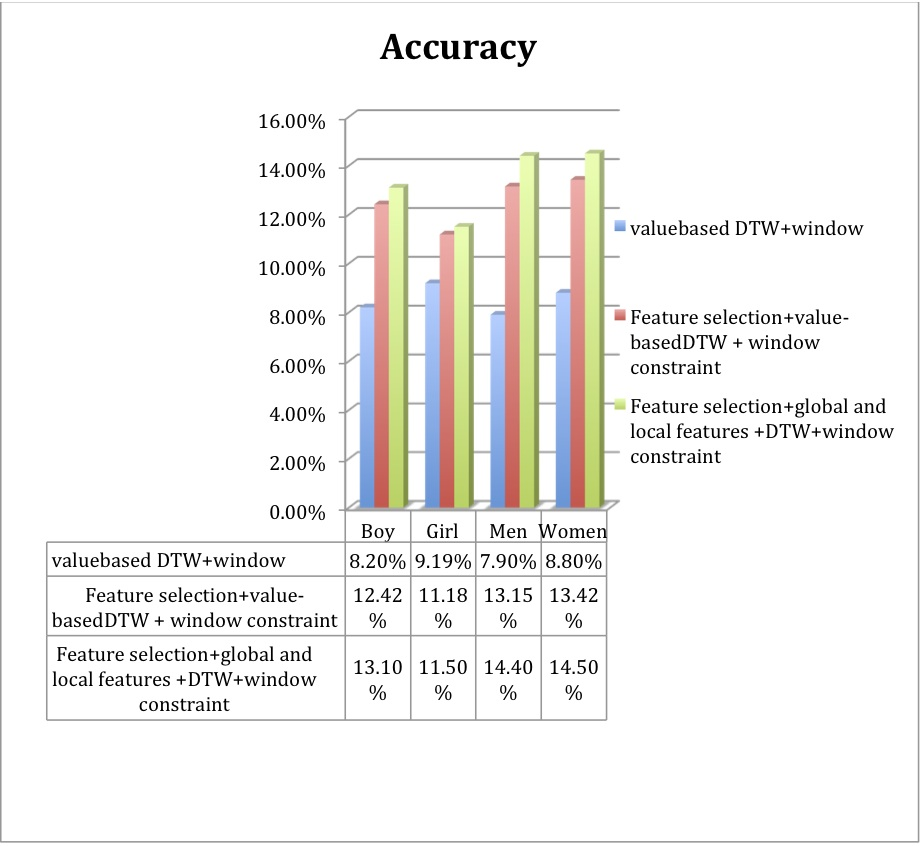
\includegraphics[scale=0.6]{localglobalaccuracy.jpg}
  \caption{}
  
\end{figure}
\begin{figure}[H]
  \centering
   
     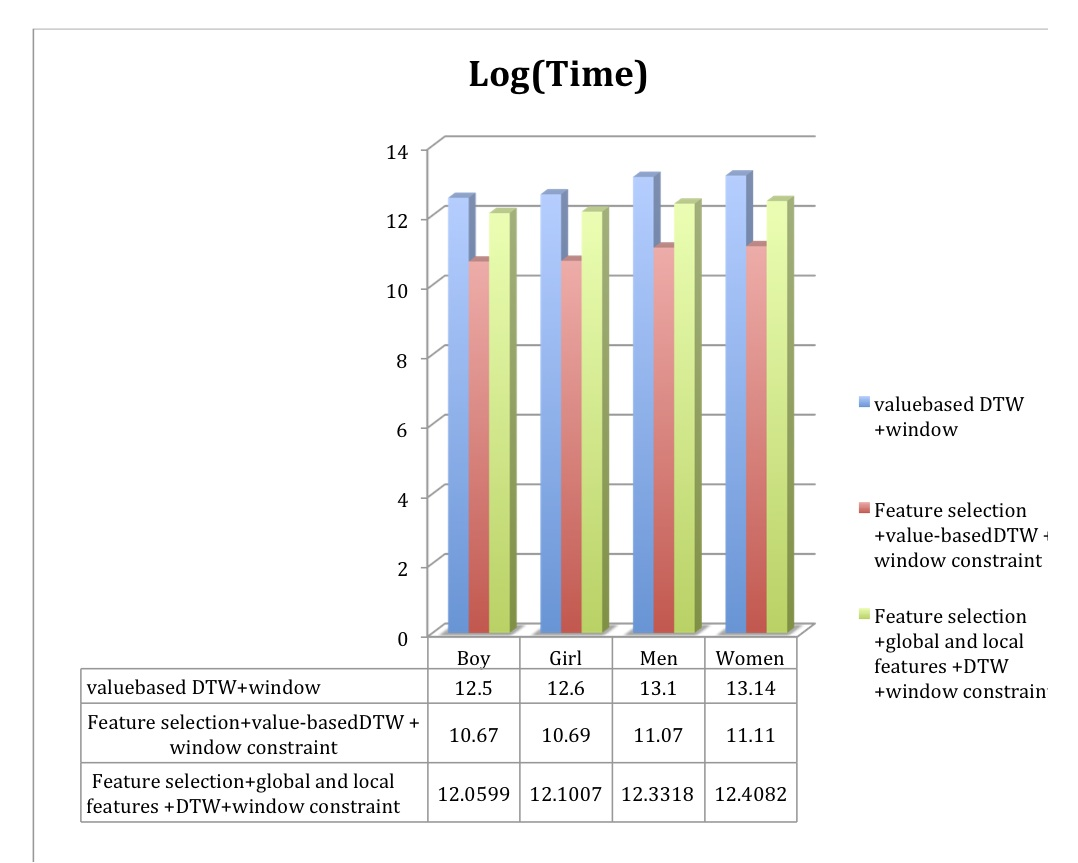
\includegraphics[scale=0.5]{localglobaltime.jpg}
  \caption{}
  
\end{figure}
Observation:
\begin{itemize}
\item Equipping DTW with a preprocessing stage that involves feature selection and extraction of local and global features result in a greater improvement in the accuracy of the algorithm.

Explanation:
\begin{itemize}
\item The algorithm now warps the time axis to  match the local and global trends  between points in the sequences instead of just their values. Since similar patterns will share the same trends, adding the feature extraction phase therefore improves the accuracy.
\end{itemize}
\item  The computational cost incurred by the algorithm is higher than the previous version that  uses  only the feature selection process.

Explanation:
\begin{itemize}
\item The cost of applying the euclidean metric on vectors $> $cost of applying the euclidean metric on points. Since the euclidean metric is applied $mn$ times. The overall computational cost increases.
\end{itemize}
\end{itemize}
The problem of working with a single data set is that if the model design is iterated many times using a limited size data set, then some over-fitting to the validation data can occur. To ensure that our model has not over fitted to the test set, I ran the two versions of DTW :one that uses the preprocessing steps of feature selection and feature extraction  while being subjected to a window constraint while the other omits  the feature extraction phase and uses the feature selection phase along with the window constraint, on the InlineSkate and Cinc\_Ecg\_Torso time series datasets[]. The results found are as follows:

\begin{figure}[H]
  \centering
   
     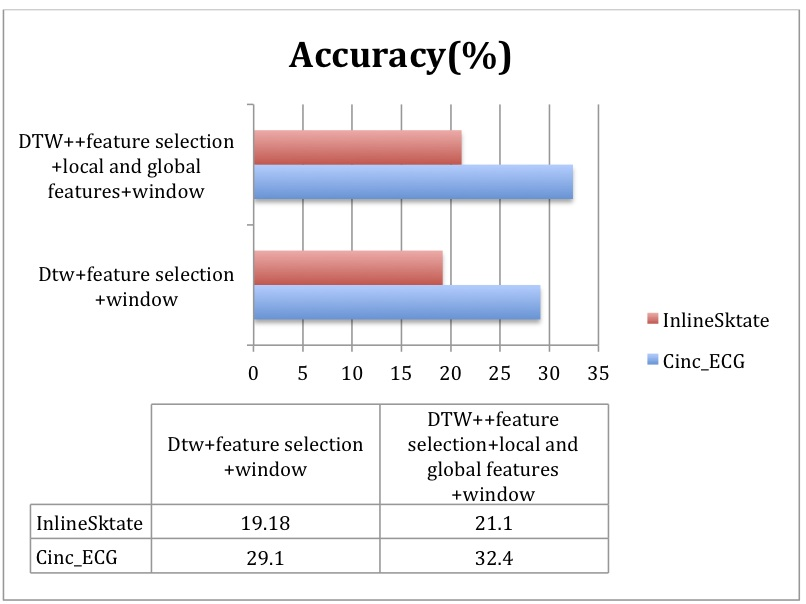
\includegraphics[scale=0.6]{cinc_inlineLocalGlobalaccuracy.jpg}
  \caption{}
  \end{figure}
\begin{figure}[H]
  \centering
   
     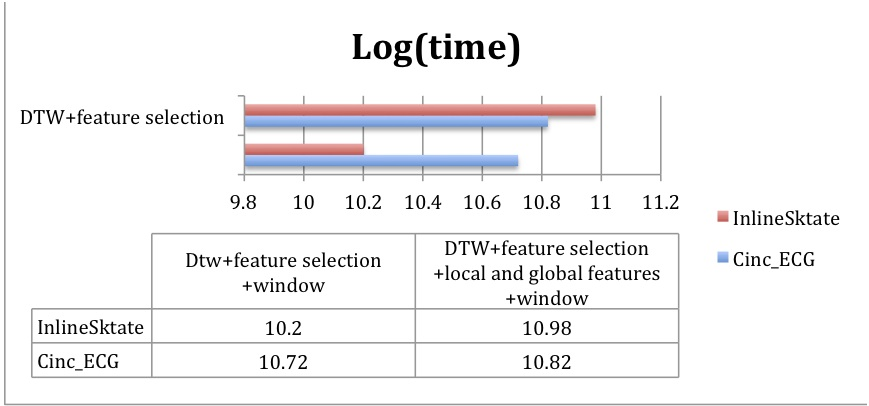
\includegraphics[scale=0.8]{cinc_inlineLocalGlobaltime.jpg}
  \caption{}
  \end{figure}
The differences between the two versions of DTW in terms of accuracy and time complexity are consistent  with the observations made in the previous experiment  with the TIDIGITS data set. This gives valid supports to the analysis of the tests that I  have conducted so far

\subsection{Domain-dependent feature extraction}

The main data set that I am working with is the TIGITS corpus which is composed of speech utterances. DTW formally is a domain independent algorithm.  It will  interesting to investigate to what degree is the  performance  of the algorithm effected if we model the information of the domain into the  DTW algorithm. Since at the moment, i am  investigating techniques that improve the performance of the DTW algorithm on high dimensional data without making changes to the algorithm itself, in this section, I investigate domain-dependent feature extraction methods that embed the  knowledge of the domain in  the feature extraction phase.  

For speech, the most commonly used features are the MFCC features-mel cepstrum ceptral coefficients.This feature representation is based on the idea of the cepstrum. For human speech, a speech waveform is created when a glottal source waveform of a particular frequency is passed through the vocal tract which because of its shape has a particular  filtering characteristic. The exact position of the vocal tract is in fact the key attribute in providing useful information about phones(units of sounds). Cepstrum provides a useful way to separate the information of the vocal tract from the glottal source.

A sketch of the MFCC feature extraction is given below:
\begin{figure}[H]
  \centering
   
     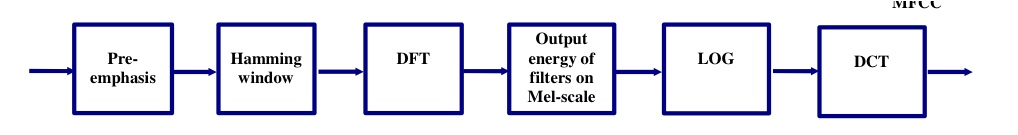
\includegraphics[scale=0.8]{mfcc.jpg}
  \caption{MFCC feature extraction}
  \end{figure}
\begin{enumerate}[label=\roman*]
\item Pre-emphasis: boosts the energy of the signal at high frequencies to improve phone detection
\item Windowing: partitions the time series sequence into frames using a hamming window
\item DFT: extracts spectral information at different frequency bands
\item Mel scale : transforming to mel scale improves recognition performance by allowing the model to take into account the property of human hearing
\item Log : makes the feature less sensitive to variations in input such as power variations on the speakers mouth.
\item Cepstrum : separate the information of the vocal tract from the glottal source. The first 12 cepstral values from spectrum of the log of the spectrum  are used
\end{enumerate}

Through the windowing process, the MFCC features extraction achieves dimensionality reduction. Each sequence is segmented into frames of length 20 to 30 ms which are then through appropriate functional mapping  are converted into sequences of MFCC feature vectors. Since the result sequence of vectors is much smaller than the length of the original sequence, the size of the DTW cost matrix is much smaller than before, This in turn lowers the time and computation cost incurred by the algorithm. One of the focal points of research for this project is to investigate alternative measures to using global window constraints that minimises the time and a computational  cost incurred by the DTW to  minimum without decreasing accuracy when working in high dimensional spaces. So  the question  that now lies is whether we can achieve greater reduction in dimensionality. The feature selection procedure that I discussed in the previous section reduces the size of the sequences by removing segments of silence followed the renaming segments by 1/2. As a prior step to MFCC feature extraction, if we use the first half of this feature selection process(i.e silence removal) and then  apply MFCC feature extraction, we achieve a dimensionality reduction which is greater than using either of the processes alone.

To test this idea I ran two versions of DTW on the TIGITS test set. The first version is equipped with a two step preprocessing stage: removal of silence followed by MFCC feature extraction while the 2nd version only employs MFCC feature extraction as pre-processing step. For this experiment, I had to impose a window constraint 
on the later version of DTW to contain the time and computational cost. Although MFCC feature extraction does achieve dimensional reduction. From doing initial tests, I have observed that the time taken by the algorithm to compare any two sequences is still  significantly high. To therefore reduce the computational time, I was forced to use the same window constraint that I employed for the previous experiments. A summary of the results of all experiments is given by the figures below:



\begin{figure}[H]
  \centering
   
     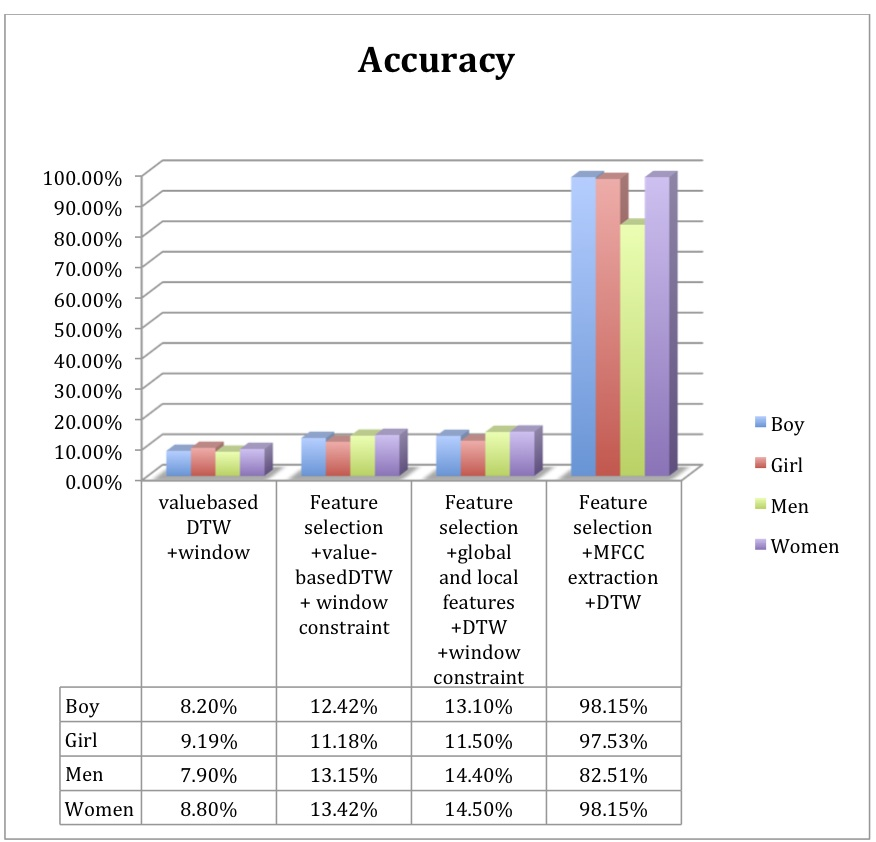
\includegraphics[scale=0.8]{Mfcc-accuracy.jpg}
  \caption{MFCC feature extraction}
  \end{figure}
  
\begin{figure}[H]
  \centering
   
     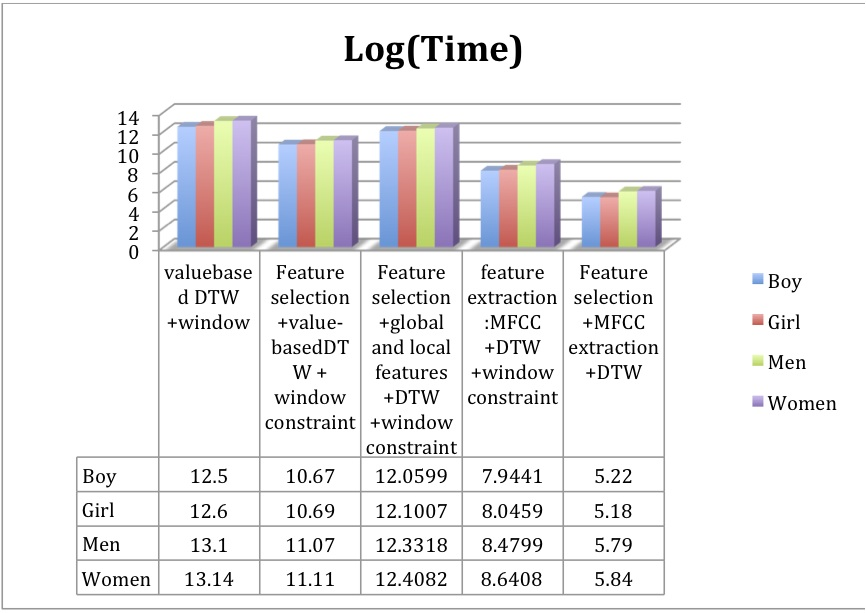
\includegraphics[scale=0.6]{Mfcc-time.jpg}
  \caption{MFCC feature extraction}
  \end{figure}
  Observations:
  \begin{itemize}
  \item It can be observed that adapting DTW to incorporate a pre-processing stage that involves removal of redundant features through silence removal and employing a feature extraction mapping that integrates domains knowledge in the feature extraction process achieves almost perfects accuracy and incurs the lowest computational time. To be precise, adapting DTW to be domain-dependent allows the algorithm to achieve near perfect accuracy while incurring the minimum computational cost. 
  \item From analysing the time complexity associated with each of the two versions, it can be seen that partitioning the sequences into frames actually leads to greater reduction in dimensionality of the time series than removing redundant features.
  \end{itemize}
  
To summarise, from the observation of the  results gathered from the  experiments it can be concluded that employing preprocessing steps that include the domain knowledge greatly improves the accuracy and time complexity of the DTW algorithm when high dimensional spaces and in some domain such the TIGITS corpus eliminates the necessity of impose global window constraints to achieve minimum computational cost.
\end{spacing}
\end{document}  